\chapter{Desarrollo de la Solución}
Dentro de esta sección se expone con precisión el procedimiento descrito previamente en la sección anterior, correspondiente a cada acción incluida en la metodología implementada, junto con los entregables previstos.

\section{Adquisición de los Datos}

\textbf{Actividad 1: Identificación de la data que contengan imágenes de rostros con características morfológicas faciales de proporciones similares}
 
Con el objetivo de entrenar un modelo de segmentación enfocado en características morfológicas faciales como arrugas y manchas, se llevó a cabo una exhaustiva búsqueda de bases de datos públicas en repositorios especializados. Se priorizó la recolección de conjuntos de datos que incluyeran imágenes faciales en alta resolución, variedad de edades, géneros y tonos de piel, así como condiciones de iluminación lo suficientemente controladas como para facilitar la segmentación de detalles faciales sutiles.

Durante este proceso, se identificaron diversos repositorios en plataformas como GitHub que ofrecían acceso a bases de datos con más de 200,000 imágenes faciales. Entre los conjuntos más destacados se encuentran versiones extendidas de datasets como CelebA, FFHQ (Flickr-Faces-HQ), y otros compendios curados por la comunidad investigadora, que contienen imágenes faciales etiquetadas o anotadas para tareas de reconocimiento y análisis facial.

Sin embargo, debido al enfoque específico de esta investigación la segmentación de características morfológicas finas como arrugas y manchas fue necesario realizar una selección cuidadosa de las imágenes más adecuadas. Para ello, se aplicaron criterios de claridad visual, resolución suficiente y visibilidad explícita de las deformaciones morfológicas faciales. Como resultado de este filtrado, se seleccionó un subconjunto compuesto por 5,000 imágenes faciales que cumplían con los siguientes criterios:

\begin{itemize}
    \item Alta calidad visual.   
    \item Visibilidad clara de texturas de la piel.
    \item Presencia evidente de arrugas y manchas.
    \item Proporciones faciales dentro de un rango estándar para facilitar el modelado.
\end{itemize} 

Este conjunto reducido pero representativo,lo podemos ver en la Figura \ref{4:fig1}, constituye la base de entrenamiento y validación del modelo propuesto. La selección manual de estos datos buscó optimizar el desempeño del modelo, al exponerlo exclusivamente a ejemplos que contienen información útil para aprender patrones asociados a las características morfológicas de interés.

\begin{figure}[h]
	\begin{center}
		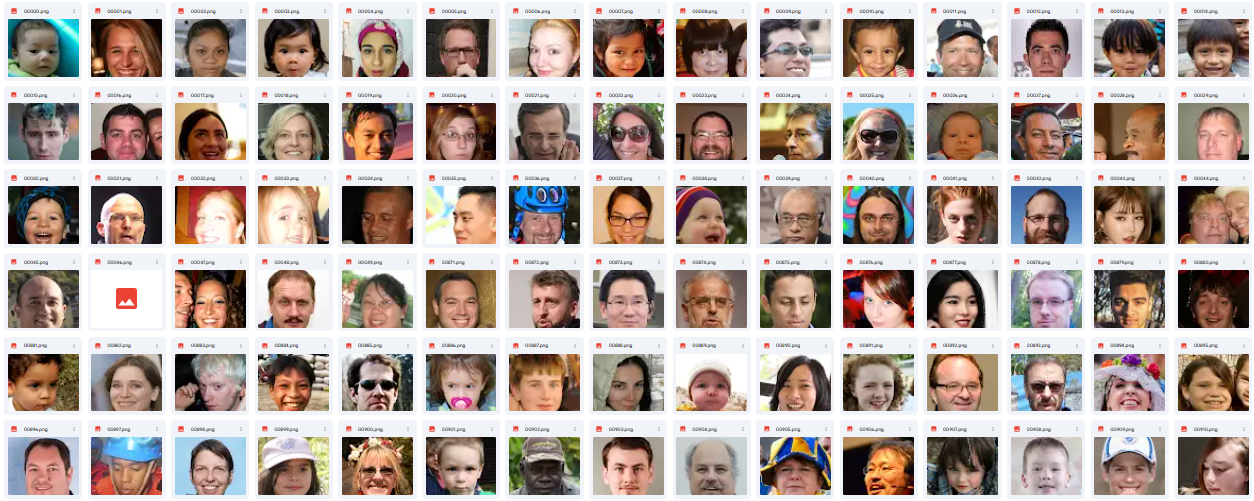
\includegraphics[width=0.75\textwidth]{4/figures/data.png}
		\caption[Dataset recolectado de repositorios]{Dataset recolectado de repositorios.\\
		Fuente: Elaboración propia}
		\label{4:fig1}
	\end{center}
\end{figure}

\section{Preprocesamiento de los Datos}

\textbf{Actividad 1: Filtración de imágenes faciales con características morfológicas}

Una vez recopilado el subconjunto de 5,000 imágenes faciales con características morfológicas visibles, se procedió a una etapa de filtración adicional orientada a reforzar la consistencia y la relevancia de los datos para la tarea de segmentación. Esta filtración se enfocó en garantizar que todas las imágenes seleccionadas contuvieran arrugas y manchas claramente identificables, descartando aquellas que, pese a su calidad visual, no presentaban estas características de manera explícita.

El proceso se realizó mediante una inspección semiautomática, apoyada en técnicas básicas de detección de texturas y realce de bordes para facilitar la identificación visual de las zonas con deformaciones. Como resultado, se aseguraron condiciones homogéneas entre las imágenes del dataset final, lo que permitió una base sólida para la generación de máscaras de segmentación precisas.

\textbf{Actividad 2: Representación y normalización de las imágenes faciales}

Con el conjunto de imágenes definitivo, se ejecutó un proceso de preprocesamiento estandarizado con dos objetivos principales: uniformar las dimensiones espaciales de las imágenes y generar las máscaras binarias asociadas a las regiones con deformaciones morfológicas.

En primer lugar, todas las imágenes fueron redimensionadas a una resolución uniforme de 1024x1024 píxeles, preservando la relación de aspecto y aplicando interpolación bilineal para mantener la calidad visual. Esta estandarización es fundamental para asegurar la compatibilidad estructural con las redes neuronales convolucionales utilizadas en etapas posteriores, y facilita la aplicación de operaciones convolucionales sobre áreas homogéneas.

En segundo lugar, se generaron máscaras binarias (en blanco y negro) correspondientes a cada imagen. Estas máscaras representan las regiones específicas del rostro que contienen arrugas, manchas u otras alteraciones morfológicas, codificadas de la siguiente manera:

\begin{itemize}
    \item Blanco (valor 1): Regiones con características morfológicas relevantes (objetivo de segmentación).   
    \item Negro (valor 0): Regiones sin interés morfológico.
\end{itemize} 

Las máscaras, como se ve en la Figura \ref{4:fig2}, fueron elaboradas a partir de una combinación de anotación semiautomática y herramientas de realce de texturas, contrastes y gradientes, con verificación manual en una muestra aleatoria para asegurar su validez.

\begin{figure}[h]
	\begin{center}
		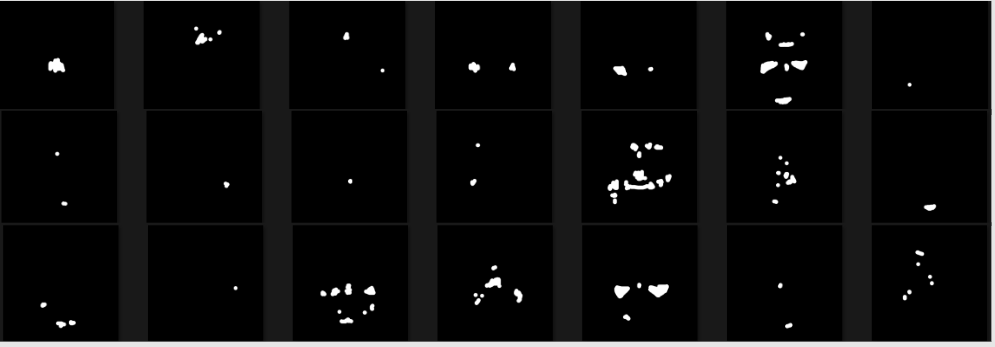
\includegraphics[width=0.75\textwidth]{4/figures/mascaras.png}
		\caption[Máscaras binarias generadas]{Máscaras binarias generadas.\\
		Fuente: Elaboración propia}
		\label{4:fig2}
	\end{center}
\end{figure}

Este proceso de representación y normalización, como se ve en el diagrama final de Preprocesamiento en la Figura \ref{4:fig3}, permitió convertir los datos originales en pares de entrada (imagen facial) y salida (máscara de segmentación), aptos para el entrenamiento supervisado del modelo de segmentación basado en redes neuronales convolucionales.

\begin{figure}[h]
	\begin{center}
		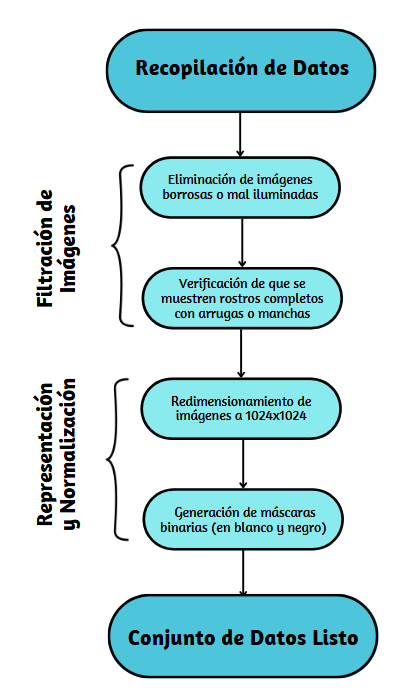
\includegraphics[width=0.75\textwidth]{4/figures/diagrama final prepo.png}
		\caption[Diagrama de Preprocesamiento Utilizado]{Diagrama de Preprocesamiento Utilizado.\\
		Fuente: Elaboración propia}
		\label{4:fig2}
	\end{center}
\end{figure}

\section{Desarrollo de los Modelos de Segmentación}

\textbf{Actividad 1: Diseño de la arquitectura del modelo}\\


La arquitectura propuesta se basa en el modelo \textbf{U-Net con mecanismos de atención} (\texttt{UNetAttention}), que combina una red convolucional simétrica tipo encoder-decoder con puertas de atención (\texttt{AttentionGate}) para mejorar el enfoque en las regiones relevantes de la imagen.

\subsection*{Encoder (Codificador)}
El encoder está diseñado para capturar características de bajo a alto nivel a partir de la imagen de entrada. Consiste en cuatro bloques llamados \texttt{DoubleConv}:
\begin{itemize}
    \item \textbf{Encoder 1}: Dos convoluciones $3\times3$ (con \texttt{padding}=1), normalización por lotes (BatchNorm) y activación ReLU. Extrae características básicas (bordes, texturas) de las entradas con 3 canales (RGB) y produce 64 mapas de características.
    \item \textbf{Encoder 2}: Similar al anterior, pero recibe 64 mapas y genera 128, aumentando la capacidad de representación.
    \item \textbf{Encoder 3}: Pasa de 128 a 256 mapas, detectando patrones más complejos.
    \item \textbf{Encoder 4}: Pasa de 256 a 512 mapas, capturando características globales.
\end{itemize}
Cada bloque está seguido de una capa \texttt{MaxPool2d(2)}, que reduce la resolución a la mitad e incrementa el campo receptivo, permitiendo captar relaciones espaciales más amplias.

\subsection*{Puente (Bottleneck)}
Entre el encoder y el decoder se encuentra el \textbf{bottleneck}, otra capa \texttt{DoubleConv} que recibe 512 mapas y genera 1024. Esta parte actúa como un resumen altamente condensado de toda la información, crucial para sintetizar las representaciones aprendidas antes de reconstruirlas.

\subsection*{Attention Gates (Puertas de Atención)}
En lugar de pasar directamente los mapas del encoder al decoder (skip connections), se introducen mecanismos de atención:
\begin{itemize}
    \item Cada \texttt{AttentionGate} recibe dos entradas: $g$ (señal del decoder) y $x$ (señal del encoder).
    \item Ambas se alinean en dimensiones espaciales y se transforman con convoluciones $1\times1$ para reducir canales.
    \item La suma de ambas se activa con ReLU, pasa por otra convolución $1\times1$, BatchNorm y una función sigmoide, generando un mapa de atención $\psi$ entre 0 y 1.
    \item Finalmente, $\psi$ se multiplica por la señal $x$ para filtrar solo las características relevantes.
\end{itemize}
Esto asegura que solo la información útil del encoder fluya al decoder, reduciendo el ruido y enfocándose en las regiones clave.

\subsection*{Decoder (Decodificador)}
El decoder reconstruye la imagen segmentada paso a paso:
\begin{itemize}
    \item \textbf{Upconv4}: Upsampling (\texttt{ConvTranspose2d}) de 1024 a 512, concatenado con la salida del encoder4 filtrado por la atención (att3).
    \item \textbf{Decoder4}: \texttt{DoubleConv} que procesa los 1024 canales concatenados y produce 512.
    \item \textbf{Upconv3}, \textbf{Decoder3}: De 512 a 256, concatenado con att2, procesado a 256.
    \item \textbf{Upconv2}, \textbf{Decoder2}: De 256 a 128, concatenado con att1, procesado a 128.
    \item \textbf{Upconv1}, \textbf{Decoder1}: De 128 a 64, concatenado con enc1 (sin atención), procesado a 64.
\end{itemize}

\subsection*{Capa Final}
La capa final es una convolución $1\times1$ que reduce los 64 mapas de características a un solo canal de salida (\texttt{out\_channels=1}), generando el mapa binario segmentado.

\subsection*{Razones del Diseño}
\begin{itemize}
    \item \textbf{Convoluciones dobles}: Mejoran la capacidad de aprendizaje local sin aumentar demasiado la profundidad.
    \item \textbf{BatchNorm}: Acelera la convergencia y estabiliza el entrenamiento.
    \item \textbf{Atención}: Permite que el modelo se enfoque en las regiones importantes, evitando pasar ruido del encoder al decoder.
    \item \textbf{Skip connections}: Ayudan a recuperar detalles espaciales perdidos por el pooling.
    \item \textbf{Puertas de atención}: Añaden un mecanismo de filtrado adaptativo, crucial en tareas donde no toda la información del encoder es igualmente relevante.
    \item \textbf{Upsampling con transposed convolutions}: Permite recuperar resolución espacial de manera más precisa que el simple escalado.
\end{itemize}

\subsection*{Detalle del Funcionamiento}
El proceso completo del modelo se detalla de la siguiente manera:
\begin{enumerate}
\item La imagen de entrada se procesa a través del encoder, extrayendo características jerárquicas que van desde bordes simples hasta patrones complejos, reduciendo la resolución pero aumentando la abstracción.
\item El bottleneck actúa como un cuello de botella que condensa toda la información del encoder en una representación compacta y de alto nivel.
\item El decoder empieza a recuperar la resolución original usando operaciones de upsampling, reconstruyendo progresivamente el mapa segmentado.
\item En cada paso del decoder, las características recuperadas se enriquecen mediante la concatenación de información relevante proveniente del encoder, filtrada cuidadosamente por las puertas de atención.
\item Las puertas de atención permiten que el modelo ignore información irrelevante y se enfoque en regiones específicas de interés para la tarea de segmentación.
\item Finalmente, la capa de salida transforma las características finales en una máscara binaria que identifica las regiones segmentadas de interés en la imagen.
\end{enumerate}

Este funcionamiento asegura que el modelo combine detalles locales finos con contexto global y mecanismos de relevancia, logrando una segmentación precisa y robusta.

\subsection*{Pseudocódigo del Modelo}
\begin{verbatim}
Input: Imagen X

# Encoder
enc1 = DoubleConv(X)
enc2 = DoubleConv(MaxPool(enc1))
enc3 = DoubleConv(MaxPool(enc2))
enc4 = DoubleConv(MaxPool(enc3))

# Bottleneck
bottleneck = DoubleConv(MaxPool(enc4))

# Decoder con atención
up4 = UpConv(bottleneck)
att3 = AttentionGate(up4, enc4)
up4_cat = Concatenate(up4, att3)
dec4 = DoubleConv(up4_cat)

up3 = UpConv(dec4)
att2 = AttentionGate(up3, enc3)
up3_cat = Concatenate(up3, att2)
dec3 = DoubleConv(up3_cat)

up2 = UpConv(dec3)
att1 = AttentionGate(up2, enc2)
up2_cat = Concatenate(up2, att1)
dec2 = DoubleConv(up2_cat)

up1 = UpConv(dec2)
up1_cat = Concatenate(up1, enc1)
dec1 = DoubleConv(up1_cat)

# Salida final
Output = Conv1x1(dec1)
Return Output
\end{verbatim}

\textbf{Actividad 2: Definición de componentes del modelo}\\
En esta actividad se definen los módulos fundamentales y los elementos de entrenamiento que constituyen el modelo UNetAttention. A continuación se describe en detalle cada uno:

\subsection*{1. Módulos arquitectónicos}

\begin{itemize}
\item \textbf{DoubleConv}:
Es un bloque formado por dos capas convolucionales secuenciales, cada una seguida de Batch Normalization y activación ReLU.
Este bloque permite:
\begin{itemize}
\item Extraer patrones locales en múltiples niveles.
\item Evitar problemas de saturación o desaparición de gradientes gracias a ReLU.
\item Estabilizar y acelerar el entrenamiento mediante BatchNorm, que normaliza las salidas y reduce la dependencia de la inicialización.
\end{itemize}

\item \textbf{AttentionGate}:
Es un módulo que implementa un mecanismo de atención espacial. Su estructura:
\begin{itemize}
\item Dos entradas: 
$\mathbf{x}$ (del encoder) y $\mathbf{g}$ (del decoder)

g (del decoder).
\item Aplicación de convoluciones 
1
×
1
1×1 para reducir dimensionalidad.
\item Suma de las dos señales transformadas y paso por activación ReLU.
\item Otra convolución 
1
×
1
1×1 seguida de BatchNorm y activación Sigmoid, que genera un mapa de atención 
\item Multiplicación punto a punto de $\psi$ con $\mathbf{x}$, filtrando las características relevantes.

x, filtrando las características relevantes.
\end{itemize}
El objetivo es permitir al modelo “enfocarse” solo en las regiones de interés para la tarea de segmentación, reduciendo ruido y mejorando la precisión espacial.

\item \textbf{UpConv (Transposed Convolution)}:
Operación que realiza upsampling aprendido, permitiendo reconstruir la resolución espacial en el decoder. Es superior al upsampling por interpolación porque también aprende qué características son importantes al expandir.

\item \textbf{Conv1x1 final}:
Capa de convolución 
1
×
1
1×1 que reduce los canales finales a uno solo (para segmentación binaria), generando la máscara final.
\end{itemize}

\subsection*{2. Componentes de entrenamiento}

\begin{itemize}
\item \textbf{Optimizador \texttt{AdamW}}:
Variante del optimizador Adam que incluye decaimiento de pesos (weight decay), lo que mejora la regularización y evita el sobreajuste. Sus ventajas incluyen:
\begin{itemize}
\item Mantenimiento de tasas de aprendizaje adaptativas por parámetro.
\item Mejor control sobre la penalización L2 (weight decay desacoplado de la actualización de momento).
\end{itemize}

\item \textbf{Scheduler \texttt{ReduceLROnPlateau}}:
Planificador que reduce la tasa de aprendizaje cuando una métrica de validación (como la pérdida) deja de mejorar después de cierto número de épocas (\textit{patience}). Esto permite:
\begin{itemize}
\item Evitar quedarse atascado en mesetas del optimizador.
\item Lograr una convergencia más fina en etapas avanzadas del entrenamiento.
\end{itemize}

\item \textbf{Función de pérdida \texttt{CrossEntropyLoss} (con pesos balanceados)}:
Se utiliza la entropía cruzada como pérdida principal para clasificación pixel a pixel. Dado que en segmentación muchas veces existe un desbalance entre clases (por ejemplo, pocas áreas afectadas vs. fondo), se aplica \textit{median frequency balancing} para calcular los pesos de cada clase, lo que:
\begin{itemize}
\item Penaliza más fuertemente los errores en clases minoritarias.
\item Mejora la sensibilidad en áreas poco representadas.
\end{itemize}
\end{itemize}

\subsection*{3. Resumen de interacción entre componentes}
Durante el entrenamiento:
\begin{enumerate}
\item El modelo recibe imágenes de entrada que son procesadas por los módulos convolucionales y de atención.
\item Las predicciones por píxel son comparadas contra las máscaras reales usando la función de pérdida ponderada.
\item El optimizador AdamW ajusta los pesos del modelo minimizando la pérdida.
\item El scheduler supervisa la evolución de la métrica de validación y adapta la tasa de aprendizaje si es necesario.
\end{enumerate}

Este conjunto de componentes fue seleccionado cuidadosamente para equilibrar capacidad, estabilidad, precisión y generalización.


\textbf{Actividad 3: Estrategia de ensamblado del modelo}\\
Se definió una estrategia de ensamblado simple basada en el entrenamiento de un solo modelo entrenado por 50 épocas, guardando el estado de mejor rendimiento en validación (menor pérdida). No se implementó ensamblado múltiple, pues la arquitectura con atención demostró ser suficiente tras el análisis de métricas.

\section{Entrenamiento del Modelo}

\textbf{Actividad 1: Configuración del entorno de entrenamiento}\\
Se configuró el entorno con los siguientes parámetros:
\begin{itemize}
  \item Ruta de datos: \texttt{face\_images}, \texttt{arrugas}, \texttt{manchas}.  
  \item Tamaño de lote (batch size): 4.  
  \item Dimensión de entrada: 256 x 256 píxeles.  
  \item Tasa de aprendizaje inicial: $1\times10^{-4}$.  
  \item Número de épocas: 50.  
  \item Dispositivo de cómputo: GPU (CUDA) o CPU según disponibilidad.  
  \item Semilla aleatoria fija (42) para reproducibilidad.  
\end{itemize}

\textbf{Actividad 2: Aplicación de técnicas de optimización}\\
Se incorporaron las siguientes técnicas:
\begin{itemize}
  \item Aumentos de datos con \texttt{albumentations}: volteos, rotaciones, ruido Gaussiano, brillo/contraste, transformaciones elásticas y desenfoque.  
  \item Balanceo de clases mediante median frequency balancing para generar pesos en \texttt{CrossEntropyLoss}.  
  \item Optimizador \texttt{AdamW} y scheduler \texttt{ReduceLROnPlateau} para ajuste automático de la tasa de aprendizaje.  
  \item Impresión de métricas de pérdida en entrenamiento y validación por época.  
\end{itemize}

\textbf{Actividad 3: Validación cruzada del rendimiento}\\
La validación se realizó con:
\begin{itemize}
  \item División de datos: 80\% entrenamiento, 20\% validación usando \texttt{train\_test\_split}.  
  \item DataLoaders separados para entrenamiento y validación, garantizando evaluación independiente.  
  \item Cálculo de métricas (pérdida, precisión, Dice, Jaccard) en el conjunto de validación cada época.  
  \item Guardado del modelo con menor \emph{val\_loss} como mejor checkpoint.  
\end{itemize}


\section{Evaluación del Modelo}

\textbf{Actividad 1: Preparación de Datos de Validación}\\
Se prepararon las imágenes de validación con transformaciones mínimas:
\begin{itemize}
  \item Redimensionamiento a 256x256 píxeles.  
  \item Conversión a tensor SIN alteraciones adicionales.  
  \item Unión de máscaras de arrugas y manchas en una única máscara multicategoría.  
\end{itemize}

\textbf{Actividad 2: Definición de Métricas de Evaluación}\\
Las métricas utilizadas fueron:
\begin{itemize}
  \item \textit{Precision} (macro) para evaluar la exactitud de las predicciones.  
  \item \textit{Dice Score} promedio para medir la superposición.  
  \item \textit{Jaccard Index (IoU)} promedio para una evaluación estricta del solapamiento.  
\end{itemize}

\textbf{Actividad 3: Evaluación del Modelo}\\
El modelo alcanzó los siguientes resultados en validación:
\begin{itemize}
  \item \textbf{Pérdida mínima (val\_loss):} 0.0458 (época 50).  
  \item \textbf{Precision promedio:} 0.645.  
  \item \textbf{Dice Score promedio:} 0.440.  
  \item \textbf{Jaccard Index promedio:} 0.289.  
  \item Se observaron mejores resultados en la detección de arrugas debido a mayor representación de esta clase.  
  \item La clase ":manchas" mostró métricas ligeramente inferiores, sugiriendo futuras mejoras en aumentos específicos.  
\end{itemize}

Los resultados numéricos y ejemplos de segmentaciones se presentan en la sección de análisis de resultados con gráficas de evolución y comparaciones visuales.


\section{Despliegue}

\textbf{Actividad 1: Preparación del Entorno de Despliegue}

\textbf{Actividad 2: Despliegue del Modelo en Producción}
